\section{Organisation}\label{sec:organization}

\noindent 
From the start in 1988 until the end of 2010, CBA was an independent entity belonging equally to Uppsala University (UU) and Swedish University of Agricultural Sciences (SLU), administered through UU. After decisions by the host universities this was changed and from 2011 the UU part of CBA became a division within the Dept.\ of Information Technology. Within the Dept. of IT, there was a review of the division structure, so from 2012 CBA together with the previous Division for Human-Computer Interaction forms the Division for Visual Information and Interaction (Vi2). Ingela Nystr\"{o}m is head of Vi2 and also head of CBA. At SLU, the Dept.~of Forest Genetics and Plant Physiology was appointed as host department where the SLU staff is employed. 

Since 2011, there is a three-year agreement between the Vice Chancellors of the two universities, according to which CBA continues as a collaboration with joint activities administered by UU. The long term strategic planning of CBA is handled by a joint council with two representatives from each university. All personnel is employed at a department at one of the two universities, and everyday management of CBA is the responsibility of the head of the division of the Dept. of IT at UU to which CBA belongs. 

The appointed members of the joint council \emph{Centrumr{\aa}d} are:
\begin{itemize}
\item Gunilla Borgefors, deputy chair, S-Faculty, SLU
\item Elna-Marie Larsson, Faculty of Medicine, UU
\item Cris Luengo, S-Faculty, SLU
\item Ingela Nystr\"{o}m, chair, TN-Faculty, UU
\end{itemize}

One component of the close integration between image analysis research at the two universities is that the SLU Professor Gunilla Borgefors is a full-time Guest Professor in computerised image processing at UU since 2012, with full financing from SLU. 

The many organizational changes in the past few years have of course affected us all, to varying degrees. We hope that the current organization will allow us to continue our successful joint research and to develop new branches with new colleagues. As seen in this report, we have been able to keep up a high activity despite a turbulent period. 

% \newpage
\subsection{Finances}
After the re-organization, where CBA at UU now is part of the Division of Visual Information and Interaction (Vi2) at the Dept.~of Information Technology, the CBA economy is not separate. 
 In fact, Vi2 has been formed to become integrated in activities as well as organization. Hence, we report how this is financed as a whole. The total expenditure for Vi2 was 39.1 million SEK for 2013. To cover this, 40\% came from UU, 8\% from SLU, 32\% from external sources, and 20\% from undergraduate education. 

The largest cost in our budget is personnel, which is 59\% of the total cost. Over the years, the number of people working at CBA has varied considerably. During 2013, about 39 people were working at CBA. Most of the personnel is employed by UU, the rest by SLU. Within the whole division Vi2, we counted more than 50 persons during the year (but not 50 full-time equivalents). 

Even though CBA itself does not organise undergraduate education, Vi2 offers undergraduate education with several courses in Human-Computer Interaction themes. In addition, we have inherited the courses on Image Analysis, Computer Graphics, and Scientific Visualization previously organised by the Division of Scientific Computing and given by teachers from CBA. Most of us teach 10--20\%, while some Senior Lecturers teach more. The economy in Table~\ref{table:balance} below summarises the overall economy for Vi2 in 2013. This summary is based on joining the two accounts from UU and SLU (after clearing internal transactions between the universities). The numbers are rounded to the nearest 1000 SEK. The same numbers for income and costs are also given as pie charts in Figure~\ref{fig:piechart}. Who finances each project can be ascertained in Section~\ref{research}, where all projects are listed. Project grants that have been received but not used are directly balanced to next year, and are thus not included in the income--cost tables.

\begin{table}[h]
\caption{Vi2 income and costs for 2014 in kSEK. \label{table:balance}}
\begin{center}
\begin{tabular}{|lr|lr|}
\hline
{\bf Income } & & {\bf Costs } & \\
\hline
UU  & 167991 & Personnel & 25081 \\
SLU & 2529 & Equipment & 99 \\
UU undergraduate education & 6476 &Operating exp.$^4$ &3175\\
Governmental grants$^1$ & 8541 & Rent & 1880 \\
Non-governmental grants$^2$ & 1253& University overhead & 9481\\
Contracts$^3$ & 4800  &  & \\
Financial netto & 44 & &\\
\hline
{\bf Total income } & {\bf 38012} & {\bf Total cost} & {\bf 39080} \\
\hline
\multicolumn{4}{l}{\small ~~~} \\
\multicolumn{4}{l}{$^1$ The Swedish Research Council, Vinnova -- Swedish Governmental Agency for Innovation Systems}\\
\multicolumn{4}{l}{$^2$ Research foundations, EU}\\
\multicolumn{4}{l}{$^3$ Internal invoices from UU and compensations}\\
\multicolumn{4}{l}{$^4$ Including travel and conferences}\\
\end{tabular}
\label{economy}
\end{center}
\end{table}

\begin{figure}[!b]
\centering

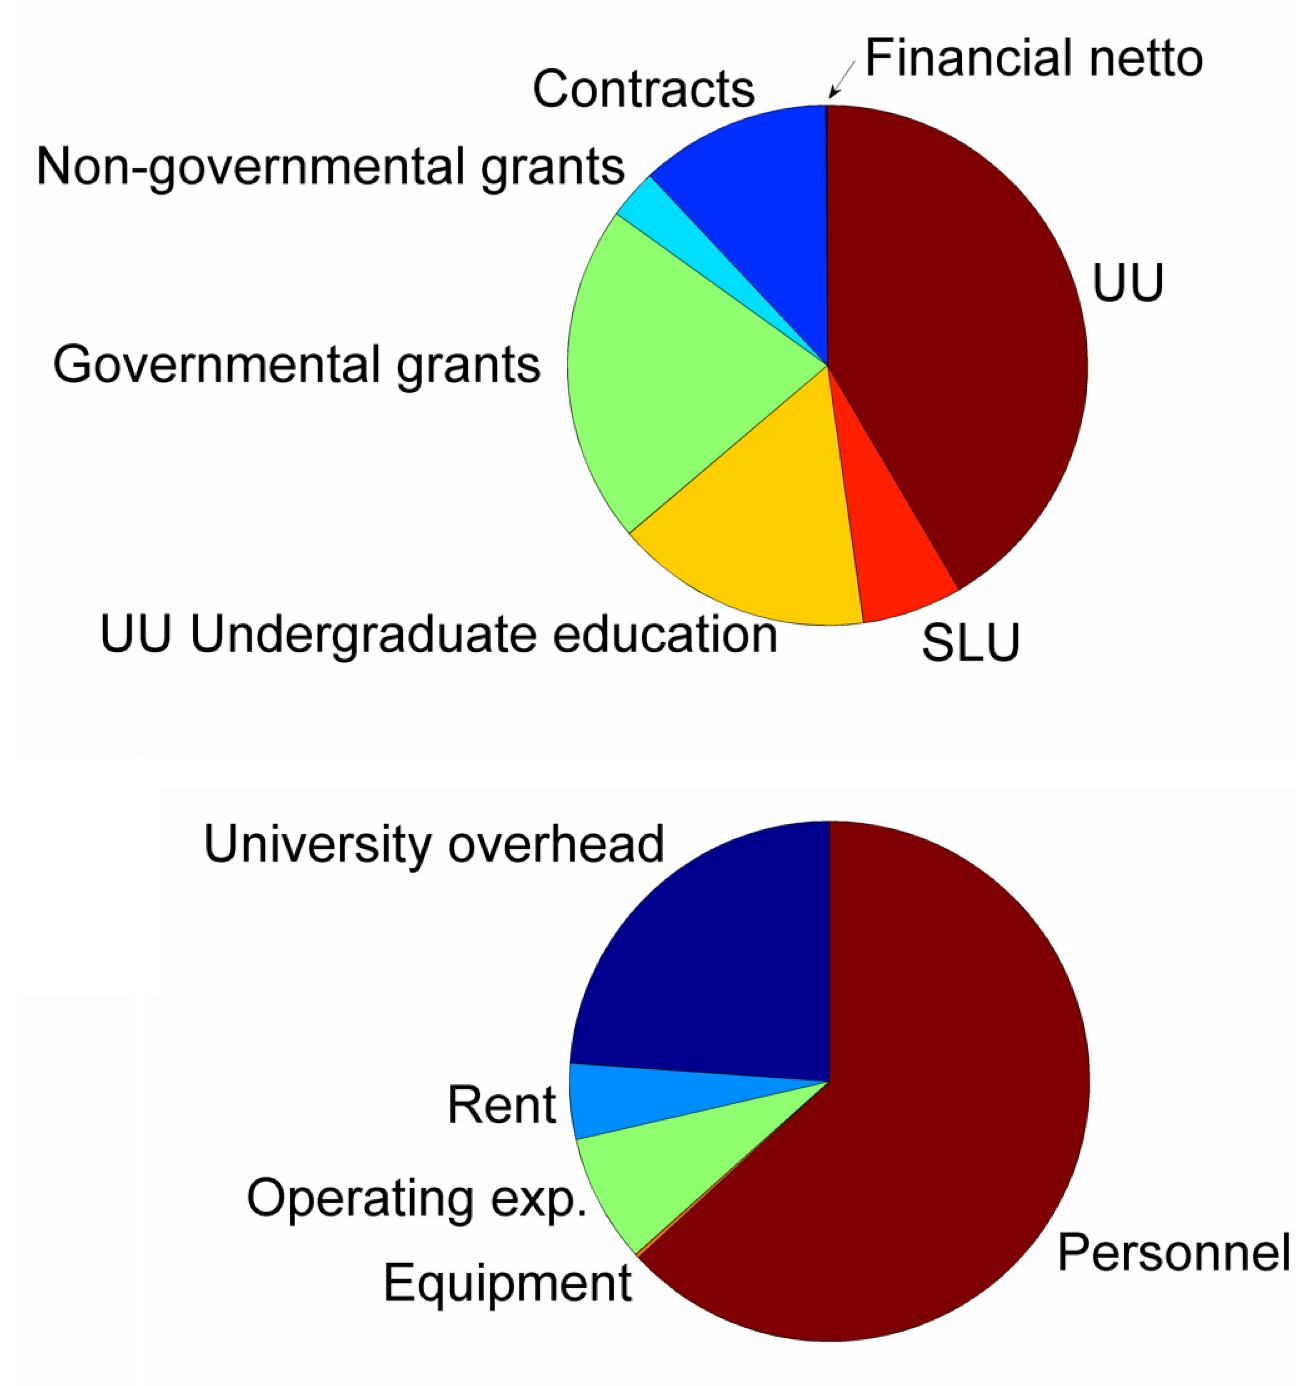
\includegraphics[width=0.65\textwidth]{./matlab/incomecost_color.png}\\

\caption{Vi2 income (top) and costs (below) for 2014.\label{fig:piechart}}
\label{Vi2incomecosts}
\end{figure}

\clearpage
\subsection{Staff, CBA}
% People who have been working in the house

\noindent
Christophe Avenel, Post Doc., UU\\
Jimmy Azar, Graduate Student --141031, UU\\
Ewert Bengtsson, Professor, UU\\
Gunilla Borgefors, Professor, UU\\
Anders Brun, PhD, Researcher, UU\\
Ingrid Carlbom, Professor, UU\\
Ginevra Castellano, Associate Senior Lecturer, 140701--\\
Vladimir Curic, Graduate Student --140831, UU\\
Olle Eriksson, PhD, Senior Lecturer, (part time) UU\\
Azadeh Fakhrzadeh, Graduate Student, SLU\\
Anders Hast, Docent and Excellent Teacher, Lecturer, UU\\
Omer Ishaq, Graduate Student, UU\\
Gustaf Kylberg, Graduate Student --140331, UU\\
Andreas K{\aa}rsn\"{a}s, Industrial Graduate Student --140430, (part time) UU and Visiopharm, H{\o}rsholm, Denmark\\
Elisabeth Linn\'er, Graduate Student, UU\\
Fei Liu, Graduate Student, University of G\"avle\\
Cris Luengo, Docent, Researcher, SLU\\
Kristina Lidayova, Graduate Student, UU\\
Patrik Malm, Graduate Student --140228, UU\\
Filip Malmberg, PhD, Researcher, UU\\
Damian Matuszewski, Graduate Student 140804--, UU\\
Bo Nordin, PhD, Researcher/Senior Lecturer, (part time) UU \\
Lena Nordstr\"{o}m, Administration\\
Fredrik Nysj\"{o}, Research Engineer, UU\\
Johan Nysj\"{o}, Graduate Student, UU\\
Ingela Nystr\"{o}m, Professor, Director, (part time) UU \\
Pontus Olsson, Graduate Student, UU\\
Alexandra Pacureanu, PhD, Post Doc --140131, UU\\
Petter Ranefall, PhD, Bioinformatician, UU\\
Sajith Sadanandan Kecheril, Graduate Student, UU\\
Kalyan Ram, Graduate Student, UU\\
Stefan Seipel, Professor, (part time) UU and University of G\"avle \\
Bettina Selig, Graduate Student, SLU\\
Ida-Maria Sintorn, Docent, Assistant Professor, SLU --140131; Associate Senior Lecturer, UU --140201\\
Natasa Sladoje, Researcher 140901--, UU\\
Robin Strand, Docent, Researcher, UU \\
Lennart Svensson, Graduate Student --141231, SLU\\
Erik Wernersson, Graduate Student --141231, SLU\\
Fredrik Wahlberg, Graduate Student, UU\\
Tomas Wilkinson, Graduate Student, UU\\
Carolina W\"{a}hlby, Docent, Senior Lecturer --140331, Professor 140401--, (part time) UU \\
\vspace*{1mm}

\noindent

\noindent
The letters after the name indicate the employer for each person:\\
UU~---~Uppsala University\\
SLU~---~Swedish University of Agricultural Sciences

%\vspace*{2mm}

\noindent
The e-mail address of the staff is {\tt Firstname.Lastname@it.uu.se}

\newpage 

\subsection*{Docent degrees from CBA}
{\small
\begin{enumerate}
\item
Lennart Thurfjell, 1999, UU
\item
Ingela Nystr\"{o}m, 2002, UU
\item
Lucia Ballerini, 2006, UU
\item 
Stina Svensson, 2007, SLU
\item
Tomas Brandtberg, 2008, UU
\item
Hans Frimmel, 2008, UU
\item
Carolina W\"{a}hlby, 2009, UU
\item
Anders Hast, 2010, UU
\item
Pasha Razifar, 2010, UU
\item
Cris Luengo, 2011, SLU
\item
Robin Strand, 2012, UU
\item
Ida-Maria Sintorn, 2012, UU
\end{enumerate}
}
\subsection*{CBA staff appointed Excellent Teachers}
{\small
\begin{enumerate}
\item
Anders Hast 2014, UU
\end{enumerate}
}
